\subsection{Code implementation}
The system is written in C\# using Microsoft Visual Studio 10. Since OpenCV\cite{opencv} is not compatible with C\# natively we use Emgu\cite{emgu} which is a wrapper for OpenCV to use in C\#. 

The design of the system has been done using UML diagrams. UML makes it easier knowing which parts communicated with other parts, their included methods and properties. The UML diagram for the PoolTracker can be seen in \ref{fig:uml}.

\begin{figure}[H]
\begin{center}
\leavevmode
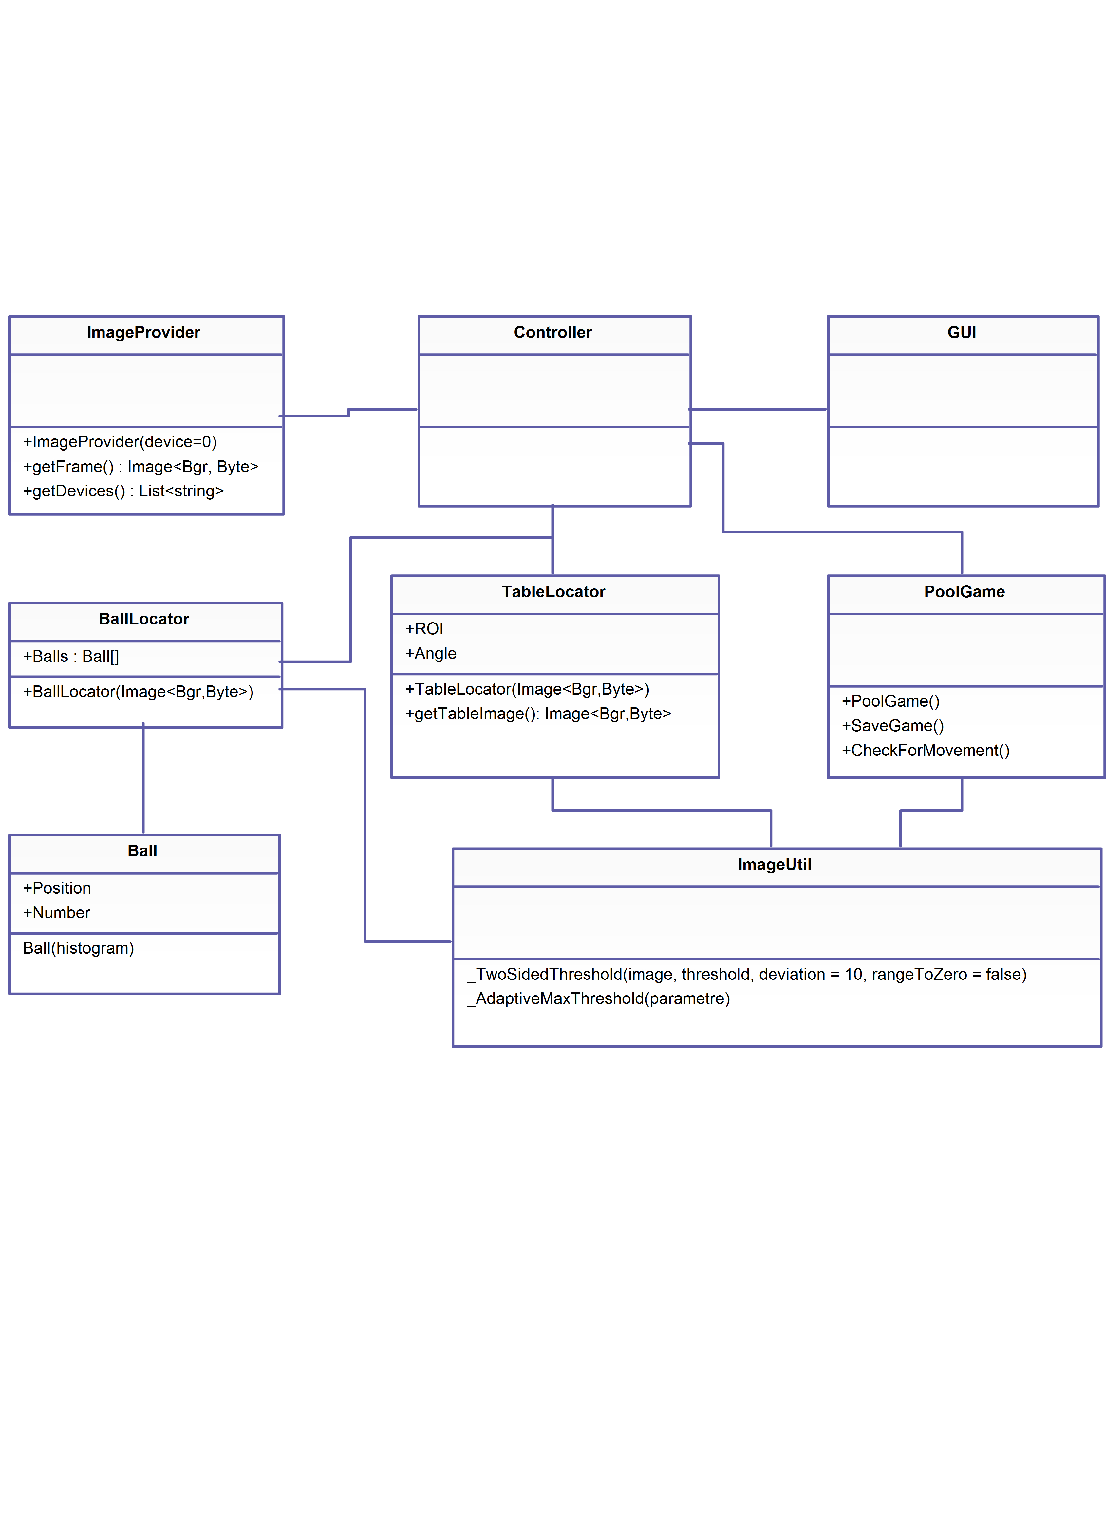
\includegraphics[width=0.8\textwidth]{images/UML}
\end{center}
\caption{UML diagram of PoolTracker.}
\label{fig:uml}
\end{figure}
